\chapter{Theory of Equations}
An equation of the form $ax^2 + bx + c = 0$, where $a, b, c\in \mathbb{C}$, the set of complex numbers, is called a \textit{quadratic
  equation}. The numbers $a, b, c$ are called \textit{coefficients} of the equation. The quantity $b^2 - 4ac$ is called the
\textit{discriminant} of the equation. It is represented by $D$ or $\Delta$. A quadratic equation represents a parabola
geometrically.

\noindent\textbf{Examples:}
\begin{enumerate}
\item $4x^2 + 4x + 1 = 0, a = 4, b = 4, c = 1$
\item $7x^3 + 10 = 0$ is not a quadratic equation.
\item $3x^2 -2x^{1/2} + 7 = 0$ is not a quadratic equation.
\item $2x^2 - 4 = 0, a = 2, b = 0, c= -4$
\end{enumerate}

The quadratic equation is called \textit{incomplete} if one of the coefficients $b$ or $c$ is zero. Thus, the last example abpve
represents an incomplete quadratic equation.

An expression of the form $ax^2 + bx + c$ is called a \textit{quadratic expression} while other elements are same as a quadratic
equation.

If two expression in $x$ are equal for all values of $x$ then this statement of equality between the two expression is called an
\textit{identity}.

$f(x) = 0$ is said to be an indentity in $x$ if it is satisfied by all values of $x$ in the domain of $f(x)$. Thus, an indentity in
$x$ is satisfied by all values of $x$ while an equation is satisfied for particular values of $x$.

\noindent\textbf{Example:} $(x + 1)^2 = x^2 + 2x + 1$ is an identity in $x$.

Two equations are called \textit{identical equations} if they have same roots.

\noindent\textbf{Example:} $x^2 - 5x + 4 = 0$ and $2x^2 - 10x + 8 = 0$ are indentical equations because both have same roots $1$ and $4$.

\noindent\textbf{Note:}
\begin{enumerate}
\item Two equations in $x$ are indentical if and only if the coefficients of similar power of $x$ in the two equations are
  proportional. Thus, if $ax^2 + bx + c = 0$ and $a_1x^2 + b_1x + c_1 = 0$ are identical equations, then $\frac{a}{a_1} =
  \frac{b}{b_1} = \frac{c}{c_1}$
\item An equation remains unchanged if it is multiplied or divided by non-zero number.
\end{enumerate}

An expression of the form $a_0x^n + a_1x^{n - 1} + a_2x^{n - 2} + \ldots + a_{n - 1}x + a_0$, where $a_0, a_1, a_2, \ldots, a_n$
are constants $(a_0 \neq 0)$ and $n$ is a positive integer is called a polynomial in $x$ of degree $n$.

As a special case a constant is also called a polynomial of degree zero.

\section{Rational Expression or Rational Function}
An expression of the form $\frac{P(x)}{Q(x)}$, where $P(x)$ and $Q(x)$ are polynomials in $x$, is called a rational expression.

In the particular case, when $Q(x)$ is a non-zero constant, $\frac{P(x)}{Q(x)}$ reduces to a polynomial.Thus, every polynomial is a
rational expression but the converse is not true.

\noindent\textbf{Examples:}
\begin{enumerate}
\item $\frac{x^2 - 5x + 4}{x - 2}$
\item $\frac{1}{x - 7}$
\end{enumerate}

\section{Roots of a Quadratic Equation}
The values $x$ for which the equation $ax^2 + bx + c = 0$ are satisfied are called roots of the equation. They are also called
roots of the quadratic expression $ax^2 + bx + c$

Every quadratic equation has at most two roots. Let $ax^2 + bx + c = 0$, where $a\neq 0$

Multiplying both sides of the equation with $a$

$a^2x^2 + abx + ac = 0 \Rightarrow (ax)^2 + 2.ax.\frac{b}{2} + \frac{b^2}{4} + ac - \frac{b^2}{4} = 0$

$\left(ax + \frac{b}{2}\right)^2 = \frac{b^2 - 4ac}{4} \Rightarrow x = \frac{-b \pm\sqrt{b^2 - 4ac}}{2a}$

These are two roots of the quadratic equation. Let us suppose the above quadratic equation has three roots $\alpha, \beta$ and
$\gamma$. These roots will satisfy the above equation. Thus,
$$a\alpha^2 + b\alpha + c = 0, a\beta^2 + b\beta + c = 0, a\gamma^2 + b\gamma + c = 0$$

Subtracting the first two, we get $(\alpha - \beta)[a(\alpha + \beta) + b] = 0$

$\because \alpha \neq \beta \therefore a(\alpha + \beta) + b = 0$

Similarly, $a(\alpha + \gamma) + b = 0$

Subtracting these two, we get $a(\alpha - \gamma) = 0$

$\because a\neq 0 \therefore \alpha = \gamma$

Thus, a quadratic equation has at most two roots.

\section{Sum and Product of the Roots}
From the two obtained  we observe that $\alpha + \beta = -\frac{b}{a}$ and $\alpha\beta = \frac{c}{a}$

\section{Nature of Roots}
For equation $ax^2 + bx + c = 0$ when $a,b,c$ are real.
\begin{enumerate}
\item When $D < 0$

  In this case, both roots will be either imaginary or complex numbers depending on whether $b$ is zero or not. These roots of
  conjugate of each other.
\item When $D = 0$

  In this case, both roots will be equal.
\item When $D > 0$

  In this case, both roots will be equal and unqual. If $D$ is not a perfect square then roots are irrational and come as a pair of
  conjugate irrational numbers.
\item When $D$ is a perfect square and $a, b, c$ are rationals.

  In this case, both roots are real and unequal.
\end{enumerate}

\subsection{Conjugate Roots}
Imaginary/complex roots of a quadratic equation with real coefficients always occur in conjugate pair.

Let $\alpha + i\beta$ be a root of the quadratic equation $ax^2 + bx + c = 0$, where $a, b, c$ are real numbers. Thus,

$a(\alpha + i\beta)^2 + b(\alpha + i\beta) + c = 0$

$\Rightarrow (a\alpha^2 - a\beta^2 + b\alpha + c) + (2a\alpha\beta + b\beta)i = 0$

Equating real and imaginary parts

$a\alpha^2 - a\beta^2 + b\alpha + c = 0, 2a\alpha\beta + b\beta = 0$

Using $\alpha - i\beta$ as the second root of the equation

$a(\alpha - i\beta)^2 + b(\alpha - i\beta) + c = (a\alpha^2 - a\beta62 + b\alpha + c) + (2a\alpha\beta + b\beta)i$

$= 0 + i.0$

Thus, we see that $\alpha - i\beta$ also satisfied the equation and is second root of the equation. Similarly, if the roots are
irrational they also appear as conjugate pair.

\section{Quadratic Expression and its Graph}
Let $f(x) = ax^2 + bx + c$, where $a, b, c\in\mathbb{R}$ and $a\neq 0$.

\begin{equation}
  \label{eq:1}
  f(x) = a\left[\left(x + \frac{b}{2a}\right)^2 + \frac{4ac - b^2}{4a^2}\right]
\end{equation}

\subsection{When a Quadratic Equation is Always Positive/Negative}
It follows from eq. \ref{eq:1}, that $f(x) > 0(< 0)~\forall~x\in\mathbb{R}$ if and only if $a > 0(< 0)$ and $D = b^2 - 4ac <
0$. See Fig. \ref{fig:1}(Fig. \ref{fig:2}). Also, it follows from \ref{eq:1} that $f(x) \geq 0(\leq 0)~\forall~x\in\mathbb{R}$ if
and only if $a > 0(< 0)$ and $D = b^2 - 4ac = 0$. in this case $f(x) < 0(< 0)$ for each $x\in R, x\neq -b/2a$, and the graph of $y
= f(x)$ touches the $x$-axis at $x = -b/2a$.

\begin{figure}[H]
  \begin{center}
    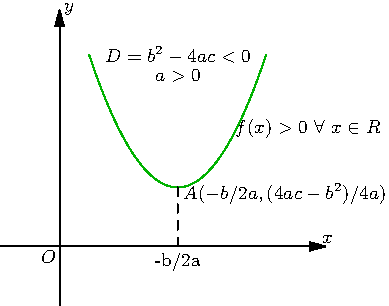
\includegraphics{quadratic-equation-1}
    \caption{When quadratic equation is always positive}
    \label{fig:1}
  \end{center}
\end{figure}

\begin{figure}[H]
  \begin{center}
    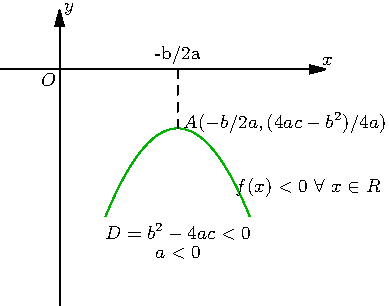
\includegraphics{quadratic-equation-2}
    \caption{When quadratic equation is always negative}
    \label{fig:2}
  \end{center}
\end{figure}

\section{Sign of a Quadratic Equation}
If $D = b^2 - 4ac > 0$, then eq. \ref{eq:1} can be written as

$$f(x) = a\left[\left(x + \frac{b}{2a}\right)^2 - \left(\frac{\sqrt{b^2 - 4ac}}{2a}\right)^2\right]$$
$$= a\left[\left(x + \frac{b + \sqrt{b^2 - 4ac}}{2a}\right)\left(x + \frac{b - \sqrt{b^2 - 4ac}}{2a}\right)\right]$$
$$= a(x - \alpha)(x - \beta)$$

If $D = b^2 - 4ac > 0$ and $a > 0$, then (See Fig. \ref{fig:3})

$$f(x) = \begin{cases}> 0\text{~for~}x <\alpha\text{~or~}x
  >\beta\\>0\text{~for~}\alpha<x<\beta\\=0\text{~for~}x=\alpha,\beta\end{cases}$$

\begin{figure}[H]
  \begin{center}
    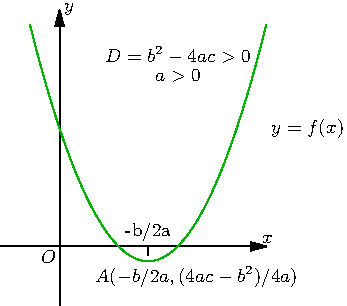
\includegraphics{quadratic-equation-3}
    \caption{When $D > 0$ and $a > 0$}
    \label{fig:3}
  \end{center}
\end{figure}

If $D = b^2 - 4ac > 0$ and $a < 0$, then (See Fig. \ref{fig:4})

$$f(x) = \begin{cases}< 0\text{~for~}x <\alpha\text{~or~}x
  >\beta\\>0\text{~for~}\alpha<x<\beta\\=0\text{~for~}x=\alpha,\beta\end{cases}$$

Note that if $a > 0$, then $f(x)$ attains the least value at $x = -b/2a$, a value which is achieved by differentiating the function
once and at this point the tangent to parabola has slope $0$. The least value is given by
$$f\left(-\frac{b}{2a}\right) = \frac{4ac - b^2}{4a}$$

If $a < 0$, then $f(x)$ is maximum at value $x = -\frac{b}{2a}$ and value of function has the same formula which is for least value
shown above.

\begin{figure}[H]
  \begin{center}
    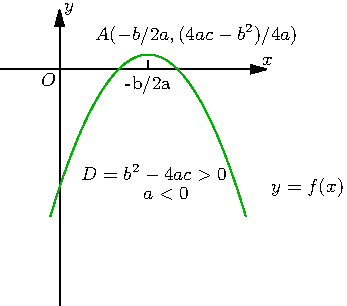
\includegraphics{quadratic-equation-4}
    \caption{When $D > 0$ and $a < 0$}
    \label{fig:4}
  \end{center}
\end{figure}

\section{Position of Roots}
\textbf{Conditions for both roots to be more than a real number $k$}

\begin{figure}[H]
  \begin{center}
    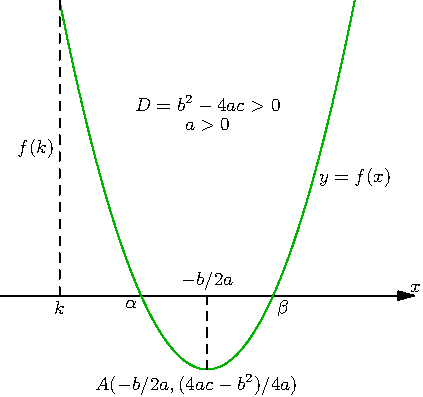
\includegraphics{quadratic-equation-5}
    \caption{When $D > 0$ and $a > 0$}
    \label{fig:5}
  \end{center}
\end{figure}

Form the Fig. \ref{fig:5}, we note that both the roots are more than $k$ if and only if $D>0,~k<-\frac{b}{2a}$ and $f(k)>0$.

In case $a< 0,$ from Fig. \ref{fig:6}, both the roots are more than $k$ if and only if $D>0,~k<-\frac{b}{2a}$ and $f(k)<0$.

\begin{figure}[H]
  \begin{center}
    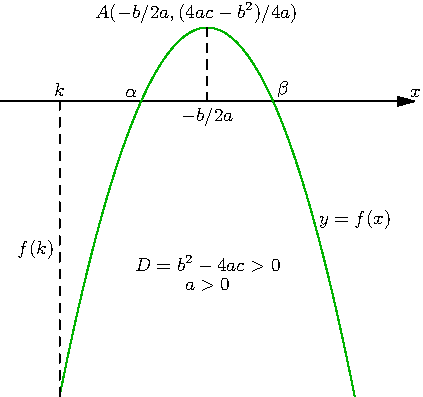
\includegraphics{quadratic-equation-6}
    \caption{When $D > 0$ and $a < 0$}
    \label{fig:6}
  \end{center}
\end{figure}

Combining the above two equations, we get the condition for the roots to be more than a real number $k$ if and only if
$D>0,~k<-\frac{b}{2a}$ and $af(k)>0$. Similarly, condition for the roots to be more than a real number $k$ if and only if
$D>0,~k>-\frac{b}{2a}$ and $af(k)>0$.

\noindent\textbf{Conditions for a real number $k$ to lie between two roots}

Similarly, the real number $k$ lies between the roots of the quadratic equation if and only if $a$ and $f(k)$ are of opposite
signs, i.e. if and only if $a>0,~D>0,~f(k) < 0$ or $a< 0,~D>0,~f(k)>0$.

Combining these two, we get $D>0,~af(k) < 0$ as the condition for $k$ to lie between two roots.

\noindent\textbf{Conditions for exactly one root to lie in between $(k_1, k_2)$ where $k_1<k_2$}

If $a>0$, then exactly one root lies in the interval $(k_1, k_2)$ if and only if $f(k_1)>0$ and $f(k_2)<0$. Also, same is true if
anad only if $f(k_1)<0$ and $f(k_2)>0$. Combining these two we get $f(k_1)f(k_2) < 0$. This condition is also true if $a<0$.

\noindent\textbf{Conditions for both roots to lie in between $(k_1, k_2)$ where $k_1<k_2$}

If $a >0$, both the roots will lies in the interval $(k_1, k_2)$ if and only if $D>0,~k_1<-\frac{b}{2a}<k_2,~f(k_1)>0$ and
$f(k_1)>0$. In case $a<0$, the conditions are $D>0,~k_1<-\frac{b}{2a}<k_2,~f(k_1)<0$ and $f(k_1)<0$.

\noindent\textbf{Conditions for the quadratic equation to have repeated roots}

The quadratic equation $f(x) = ax^2 + bx + c = 0, a\neq 0$ has a repeated root if and only if $f(\alpha) = f'(\alpha) = 0$, where
$\alpha$ is the repeated root. In this case, $f(x) = a(x - \alpha)^2$, In fact, $\alpha = -b/2a$. Geometrically, the $x$-axis will
be a tangent to the parabola at $x = -b/2a$. See Fig. \ref{fig:7} and Fig. \ref{fig:8}.

\begin{figure}[H]
  \begin{center}
    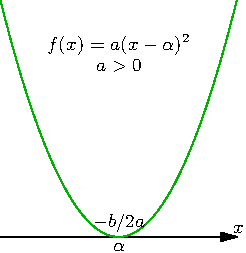
\includegraphics{quadratic-equation-7}
    \caption{$f(\alpha)=0,~f'(\alpha)=0$}
    \label{fig:7}
  \end{center}
\end{figure}

\begin{figure}[H]
  \begin{center}
    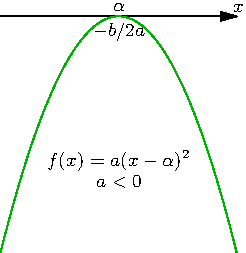
\includegraphics{quadratic-equation-8}
    \caption{$f(\alpha)=0,~f'(\alpha)=0$}
    \label{fig:8}
  \end{center}
\end{figure}

\noindent\textbf{Conditions for two quadratic equations to have one common root}

Consider two quadratic equations $ax^2 + bx + c = 0$ and $a'x^2 + b'x^2 + c' = 0$ having a common root $\alpha$. Clearly, this
common root will satisfy both the equations, i.e. $a\alpha^2 + b\alpha + c = 0$ and $a'\alpha^2 + b'\alpha + c' = 0$.

Solving these two equations, we get

$$\frac{\alpha^2}{bc' - b'c} = \frac{\alpha}{a'c - ac'} = \frac{1}{ab' - a'b}$$
$$\Rightarrow \alpha^2 = \frac{bc' - b'c}{ab' - a'b}, \alpha = \frac{a'c - ac'}{ab' - a'b}$$

Eliminating $\alpha$, we get

$$(a'c - ac')^2 = (bc' - b'c)(ab' - a'b)$$

This is the required condition for two quadratic equations to have one common root.

\begin{figure}[H]
  \begin{center}
    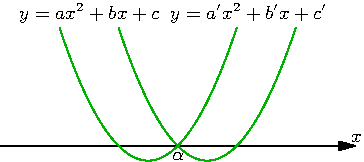
\includegraphics{quadratic-equation-9}
    \caption{Common roots}
    \label{fig:9}
  \end{center}
\end{figure}

\begin{figure}[H]
  \begin{center}
    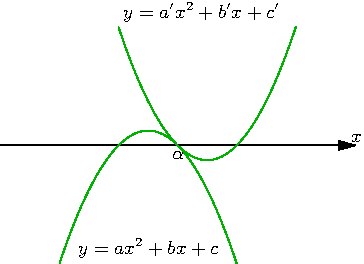
\includegraphics{quadratic-equation-10}
    \caption{Common roots}
    \label{fig:10}
  \end{center}
\end{figure}

To obtain the common root make coefficients of $x^2$ in both the equations same and subtract one equation from the other to obtain
a linear equation in $x$, which you can solve to obtain the common root.

For having both roots common the two equations must be identical i.e. $\frac{a}{a'} = \frac{b}{b'} = \frac{c}{c'}$

\section{General Quadratic Equation in $x$ and $y$}
The general quadratic equation in $x$ and $y$ is given by $ax^2 + 2hxy + by^2 + 2gx + 2fy + c = 0$

$$\therefore x = \frac{-2(hy + g)\pm\sqrt{4(hy + g)^2 - 4a(by^2 + 2fy + c)}}{2a}$$
$$\Rightarrow x + hy + g = \pm \sqrt{(h^2 - ab)y^2 + 2(gh - af)y + g^2 - ac}$$

It can be resolved into two linear factors if $(h^2 - ab)y^2 + 2(gh - af)y + g^2 - ac$ is a perfect square and $h^2 - ab > 0$.

The condition for $(h^2 - ab)y^2 + 2(gh - af)y + g^2 - ac$ to be a perfect square is that its discriminant is $0$, i.e.

$$4(gh - af)^2 - 4(h^2 - ab)(g^2 - ac) = 0$$
$$\Rightarrow abc + 2fgh - af^2 - bg^2 - ch^2 = 0$$

\section{Equations of Higher Degree}
The equation $f(x) = a_0x^n + a_1x^{n - 1} + a_2x^{n - 2} + \ldots + a_{n - 1}x + a_n = 0$, where $a_0, a_1 \ldots,
a_n\in\mathbb{C}$, the set of complex numbers and $a_0\neq 0$, is said to be an equation of degree $n$. An equation of degree $n$
has exactly $n$ roots. Let $\alpha_1, \alpha_2, \ldots, \alpha_n\in\mathbb{C}$ be the $n$ roots. Then
$$f(x) = a_0(x - \alpha_1)(x - \alpha_2)\ldots(x - \alpha_n)$$
$$\sum\alpha_i = -\frac{a_1}{a_0}, \sum\alpha_i\alpha_j = \frac{a_2}{a_0}, \ldots, \prod\alpha_i = (-1)^n\frac{a_n}{a_0}$$

\section{Cubic and Biquadratic Equation}
If $\alpha, \beta, \gamma$ are the roots of $ax^3 + bx^2 + cx + d = 0$, then
$$\alpha + \beta + \gamma = -\frac{b}{a}, \alpha\beta + \beta\gamma + \gamma\alpha = \frac{c}{a}, \alpha\beta\gamma =
-\frac{d}{a}$$

Also, if $\alpha, \beta, \gamma, \delta$ are the roots of the equation $ax^4 + bx^3 + cx^2 + d + e = 0$, then
$$\alpha + \beta + \gamma + \delta = -\frac{b}{a}, \alpha\beta + \alpha\gamma + \alpha\delta + \beta\gamma + \beta\delta +
\gamma\delta = \frac{c}{a}$$
$$\alpha\beta\gamma + \alpha\beta\delta + \alpha\gamma\delta + \beta\gamma\delta = -\frac{d}{a}, \alpha\beta\gamma\delta =
\frac{e}{a}$$

\section{Transformation of Equations}
Let the given equation be

\begin{equation}
  \label{eq:2}
  f(x) = a_0x^n + a_1x^{n - 1} + a_2x^{n - 2} + \ldots + a_{n - 1}x + a_n = 0
\end{equation}
\begin{enumerate}
\item To form an equation whose roots are $k(\neq 0)$ times roots of the eq. \ref{eq:2}, replace $x$ by $x/k$.
\item To form an equation whose roots are the negatives of the roots of eq. \ref{eq:2}, replace $x$ by $-x$. Alternatively, change
  the sign of the coefficients of $x^{n - 1}, x^{n - 3}, x^{n - 5}, \ldots$ etc. in \ref{eq:2}.
\item To form an equation whose roots are $k$ more than the roots of eq. \ref{eq:2}, replace $x$ by $x - k$ in \ref{eq:2}.
\item to form an equation whose roots are reciprocals of roots in eq. \ref{eq:2}, replace $x$ by $1/x$ in \ref{eq:2} and then
  multiply both sides by $x^n$.
\item To form an equation whose roots are squares of roots in eq. \ref{eq:2}, replace $x$ by $\sqrt{x}$. Then you can collect all
  terms involving $\sqrt{x}$ on one side and square both sides followed by simplification.
\item To form an equation whose roots are cubes of roots in eq. \ref{eq:2}, replace $x$ by $\sqrt[3]{x}$. Then you can collect all
  terms involving $\sqrt[3]{x}$ and $\sqrt[3]{x^2}$ on one side and cube both sides followed by simplification.
\end{enumerate}

\section{Descartes Rule}
\begin{enumerate}
\item[Rule 1:] The maximum no. of positive real roots of eq. \ref{eq:2} is the number of changes of sign of coefficients from
  positive to negative and negative to positive.
\item[Rule 2:] The maximum no. of negtive real roots of eq. \ref{eq:2} is the number of changes of sign of coefficients from
  positive to negative and negative to positive in the equation $f(-x) = 0$.
\end{enumerate}

\section{Hints for Solving Polynomial Equations}
\begin{enumerate}
\item To solve the equation of the form $(x - a)^{2n} + (x - b)^{2n} = A$, where $n\in\mathbb{P}$, put $y = x - \frac{a + b}{2}$.
\item To solve the equation of the form $a_0(f(x))^{2n} + a_1(f(x))^{n} + a_2 = 0$, put $(f(x))^n = y$ then we obtain two roots
  $y_1, y_2$ to solve again for $f(x) = y_1, f(x) = y_2$.
\item An equation of the form $(ax^2 + bx + c_1)(ax^2 + bx + c_2)\ldots(ax^2 + bx + c_n) = A$ can be solved by putting $ax^2 + bx =
  y$.
\item An equation of the form $(x - a)(x - b)(x - c)(x - d) = Ax^2$, where $ab = cd$, can be reduced to a product of two quadratic
  polynomials by putting $y = x + \frac{ab}{x}$.
\item An equation of the form $(x - a)(x - b)(x - c)(x - d) = A$, where $a<b<c<d, b - a = d - c$ can be solved by putting $y = x -
  \frac{a + b + c + d}{4}$.
\item A polynomial $f(x, y)$ is said to be symmetric if $f(x, y) = f(y, x)~\forall~x, y$. All symmetric polynomials can be
  represented as a function of $x + y$ and $xy$.
\end{enumerate}

\section{Problems}
\begin{enumerate}
\item For what values of $(1 + m)x^2 - 2(1 + 3m)x + (1 + 8m) = 0$ has equal roots?
\item If $a + b + c = 0$ and $a,b,c$ are rational. Prove that the roots of the equation $(b + c - a)x^2 + (c + a - b)x + (a + b -
  c) = 0$ are rational.
\item Show that if the roots of the equation $(a^2 + b^2)x^2 + 2(ac + bd)x + c^2 + d^2 = 0$ are real, they will be equal.
\item If the roots of the equation $a(b - c)x^2 + b(c - a)x + c(a - b) = 0$ be equal, prove that $a, b, c$ are in H.P.
\item If $a + b + c = 0$ and $a,b,c$ are real, prove that equation $(b - x)^2 - 4(a - x)(c - x) = 0$ has real roots and roots will
  not be equal unless $a=b=c$.
\item Show that if $p,q,r,s$ are real numbers and $pr = 2(q + s)$ then at least one of the equations $x^2 + px + q = 0$ and $x^2 +
  rx + s = 0$ has real roots.
\item If the equation $x^2 - 2px + q = 0$ has two equal roots, then the equation $(1 + y)x^2 - 2(p + y)x + (q + y) = 0$ will have
  its roots real and distinct only when $y$ is negative and $p$ is not unity.
\item If the equation $ax^2 + 2bx + c = 0$ has real roots. $a,b,c$ being real numbers and if $m$ and $n$ are real numbers such that
  $m^2 > n^2 > 0$ then prove that the equation $ax^2 + 2mbx + nc = 0$ has real roots.'
\item If theq equations $ax + by = 1$ and $cx^2 + dy^2 = 1$ have only one solution, prove that $\frac{a^2}{c} + \frac{b^2}{d} = 1$
  and $x = \frac{a}{c}, y = \frac{b}{d}$.
\item If $r$ be the ratio of the roots of the equation $ax^2 + bx + c = 0,$ show that $\frac{(r + 1)^2}{r} = \frac{b^2}{ac}$.
\item If one root of the eq. $(l - m)x^2 + lx + 1 = 0$ be double of the other and if $l$ be real, show that $m\leq \frac{9}{7}$.
\item If one root of the quadratic equation $ax^2 + bx + c = 0$ is equal to the $n$th power of the other, then show that
  $$(ac^n)^{1/(n + 1)} + (a^nc)^{1/(n + 1)} + b = 0$$
\item If the roots of the equation $ax^2 + bx + c = 0$ be in the ratio $p:q$, show that
  $$\sqrt{\frac{p}{q}} + \sqrt{\frac{q}{p}} + \sqrt{\frac{c}{a}} = 0$$
\item If $\alpha$ and $\beta$ be the roots of the equation $x^2 + px + q = 0$. Find the value of the following in the terms of $p$
  and $q$.
  \begin{enumerate}
  \item $\frac{\alpha^2}{\beta} + \frac{\beta^2}{\alpha}$
  \item $(\omega\alpha + \omega^2\beta)(\omega^2\alpha + \omega\beta)$, where $\omega$ an imaginary cube root fo unity.
  \end{enumerate}
\item If $\alpha$ and $\beta$ be the roots of the equation $A(x^2 + m^2) + Amx + cm^2x^2 = 0$, prove that $A(\alpha^2 + \beta^2) +
  A\alpha\beta + c\alpha^2\beta^2 = 0$.
\item If $\alpha$ and $\beta$ be the roots of the euqation $ax^2 + bx + c = 0$, prove that $a\left(\frac{\alpha^2}{\beta} +
  \frac{\beta^2}{\alpha}\right) + b\left(\frac{\alpha}{\beta} + \frac{\beta}{\alpha}\right) = b$.
\item If $a$ and $b$ are the roots of the equation $x^2 + px + 1 = 0$ and $c$ and $d$ are the roots of the equation $x^2 + qx + 1 =
  0$, show that $q^2 - p^2 = (a - c)(b - c)(a + d)(b + d)$.
\item If the roots of the equation $x^2 + px + q = 0$ differ from the roots of the equation $x^2 + qx + p = 0$ by the same
  quantity, show that $p + q + 4 = 0$.
\item If $\alpha, \beta$ are the roots of the equation $ax^2 + bx + c = 0$ and $S_n = \alpha^n + \beta^n$, show that $aS_{n + 1} +
  bS_n + cS_{n - 1} = 0$ and hence find $S_5$.
\item If the sum of roots of the equation $ax^2 + bc + c = 0$ is equal to the sum of the squares of their reciprocals, show that
  $bc^2, ca^2, ab^2$ are in A.P.
\item If $\alpha$ and $\beta$ be the values of $x$ obtained from the equation $m^2(x^2 - x) + 2mx _ 3 = 0$ and if $m_1$ and $m_2$
  be the two values of $m$ for which $\alpha$ and $\beta$ are connected by the relation $\frac{\alpha}{\beta} +
  \frac{\beta}{\alpha} = \frac{4}{3}$, find the value of $\frac{m_1^2}{m_2} + \frac{m_2^2}{m_1}$.
\item If the ratio of the roots of the equation $ax^2 + bx + c = 0$ be equal to the roots of equation $a_1x^2 + b_1x + c_1 = 0$,
  prove that $\left(\frac{b}{b_1}\right)^2 = \frac{ca}{c_1a_1}$.
\item Find the quantity equation with the rational coefficients one of whose roots is $\frac{1}{2 + \sqrt{5}}$.
\item If $\alpha$ and $\beta$ be the roots of the equation $ax^2 + bx + c = 0$, find the quantity equation whose roots are
  $\frac{1}{a\alpha + b}$ and $\frac{1}{a\beta + b}$.
\item If $c, d$ are the roots of the equation $(x - a)(x - b) = k$, show that $a,b$ are the roots of the equation $(x - c)(x - d) +
  k = 0$
\item The coefficients of $x$ in the equation $x^2 + px + q = 0$ was wrongly written as $17$ in place of $13$ and roots were found
  to be $-2$ and $-15$. Find the roots of the correct equation.
\item If $\alpha$ and $\beta$ be the roots of the equation $x^2 + px + q = 0$, show that $\frac{\alpha}{\beta}$ is a root of the
  equation $qx^2 - (p^2 - 2q)x + q = 0$.
\item If $x^2 - ax + b = 0$ and $x^2 - px + q = 0$ have a common root and the second equation has equal roots then show that $b + q
  = \frac{ap}{2}$.
\item If $ax^2 + 2bx + c = 0$ and $a_1x^2 + 2b_1x + c_1 = 0$ have a common root and $\frac{a}{a_1}, \frac{b}{b_1}, \frac{c}{c_1}$
  are in A.P., show that $a_1, b_1, c_1$ are in G.P.
\item If each pair of the followingf three equations $x^2 + p_1x + q_1 = 0, x^2 + p_2x + q_2 = 0, x^2 + p_3x + q_3 = 0$ have
  exactly one root in common, then show that $(p_1 + p_2 + p_3)^2 = 4(p_1p_2 + p_2p_3 + p_3p_1 - q_1 - q_2 - q_3)$.
\item If the equations $x^2 + cx + bc = 0$ and $x^2 + bx + ca = 0$ have a common root, show that $a + b + c = 0$; show that other
  roots are given by the equation $x^2 + ax + bc = 0$.
\item If $a, b, c\in\mathbb{R}$ and equations $ax^2 + bx + c = 0$ and $x^2 + 2x + 9 = 0$ have a common root, show that $a:b:c =
  1:2:9$.
\item Find the value of $p$ if the equation $3x^2 - 2x + p = 0$ and $6x^2 - 17x + 12 = 0$ have a common root.
\item Show that $|x|^2 - |x| - 2 = 0$ is an equation.
\item Show that $\frac{(x + b)(x + c)}{(b - a)(c - a)} + \frac{(x + c)(x + a)}{(c - b)(a - b)} + \frac{(x + a)(x + b)}{(a - c)(b -
  c)} = 1$ is an indenity.
\item If $a, b, c, a_1, b_1, c_1$ are rational and equations $ax^2 + 2bx + c = 0$ and $a_1x^2 + 2b_1x + c_1 = 0$ have one and only
  one root in common, prove that $b^2 - ac$ and $b_1^2 - a_1c_1$ must be perfect squares.
\item If $(a^1 - 1)x^2 + (a - 1)x + a^2 - 4a + 3 = 0$ be an indentity in $x$, then find the value of $a$.
\item Solve $\left(x + \frac{1}{x}\right)^2 = 4 + \frac{3}{2}\left(x + \frac{1}{x}\right)$.
\item Solve $(x + 4)(x + 7)(x + 8)(x + 11) + 20 = 0$.
\item Solve $3^{2x + 1} + 3^2 = 3^{x + 3} + 3^x$.
\item Solve $(5 + 2\sqrt{6})^{x^2 - 3} + (5 - 2\sqrt{6})^{x^2 - 3} = 10$.
\item A car travels $25$ km per hour faster than a bus for a jouney of $500$ km. The bus takes $10$ hours more than the car. Find
  the speed of the bus and the car.
\item Show that the roots of the equation $(a + b)^2x^2 - 2(a^2 - b^2)x + (a - b)^2 = 0$ are equal.
\item Show that the equation $3x^2 + 7z+ 8 = 0$ cannot be satisfied by any real values of $x$.
\item For what values of $a$ will the roots of the equation $3x^2 + (7 + a)x + 8 - a = 0$ be equal.
\item If the roots of the equation $(a^2 + b^2)x^2 + 2(ac + bd)x + (c^2 + d^2) = 0$ are equal then show that $a:b = c:d$.
\item Prove that the roots of the equation $(b - c)x^2 + 2(c - a)x + (a - b) = 0$ are always real.
\item Show that the roots of the equation $\frac{1}{x - a} + \frac{1}{a} + \frac{1}{x - 1} = 0$ are real for all real values of
  $a$.
\item Show that if $a + b + c = 0$, the roots of the equation $ax^2 + bx + c = 0$ are rational.
\item Prove that the roots of the equation $(b + c - 2a)x^2 + (c + a - 2b)x + (a + b - 2c) = 0$ are rational.
\item Show that the roots of the equation $x^2 + rx + s = 0$ will be rational if $r = k + \frac{s}{k}$, where $r, s$ and $k$ are
  rational.
\item Prove that roots of the equation $(x - a)(x - b) + (x - b)(x - c) + (x - c)(x - a) = 0$ are always real and cannot be equal
  unless $a = b = c$.
\item If $a, b, c$ are rational, show that the roots of the equation $a^2(b^2 - c^2)x^2 + b^2(c^2 - a^2)x + c^2(a^2 - b^2) = 0$ are
  rational.
\item Show that the roots of the equation $(a^4 + b^4)x^2 + 4abcdx + c^4 + d^4 = 0$ cannot be different, if real.
\item If $p, q, r$ are in H.P. and $p$ and $r$ are of the same sign, prove that the roots of the equation $px^2 + 2qx + r = 0$ will
  be complex.
\item Prove that the roots of the equation $bx^2 + (b - c)x + (b - c - a) = 0$ are real if those of equation $ax^2 + 2bx + b = 0$
  are imaginary and vice-versa.
\item Prove that the values of $x$ obtained from the equations $ax^2 + by^2 = 1$ and $ax + by = 1$ will be equal if $a + b = 1$.
\item Prove that the values of $x$ obtained from the equations $x^2 + y^2 = a^2$ and $y = mx + c$ will be equal if $c^2 = a^2(1 +
  m^2)$.
\item The roots of the equation $4x^2 - (5a + 1)x + 5a = 0$ are $\alpha$ and $\beta$. If $\beta = 1 + \alpha$, calculate the
  possible values of $a, \alpha$ and $\beta$.
\item If one root of the equation $5x^2 + 13x + k = 0$ be reciprocal of another, find $k$.
\item Find the values of $m$, for which the equation $5x^2 - 4x + 2 + m(4x^2 - 2x - 1) = 0$ has (a) equal roots, (b)the products of
  root is $2$, and (c) the sum of roots is $6$.
\item Find the relation between the coefficients of the quadratic equal $ax^2 + bx + c = 0$ if one root is $n$ times the another.
\item If the roots of the equation $ax^2 + bx + c = 0$ are in the ratio $3:4$, prove that $12b^2 = 49ac$.
\item If the roots of the equation $4x^2 + ax + 3 = 0$ are in the ratio $1:2$, show that the roots of the equation $ax^2 + 3x + a =
  2$ are imaginary.
\item If one root of the equation $x^2 - px + q = 0$ be $m$ times their difference, prove that $p^2(m^2 - 1) = 4m^2q$.
\item If the difference of the roots $x^2 - px + q = 0$ is unity, then prove that $p^2 - 4q = 1$ and $p^2 + 4q = (1 + 2q)^2$.
\item Find the condition that the equation $\frac{a}{x - a} + \frac{b}{x - b} = m$ may have roots equal in magnitude but opposite
  in sign.
\item Find the relation between coefficients of the euqation $ax^2 + bx + c = 0$ if one root exceeds other by $k$.
\item If one root of the equation $ax^2 + bx + c = 0$ be square of the other, show that $b^3 + a^2c + ac^2 = 3abc$.
\item Determine the value $p$ for which one root of the equation $x^2 + px + 1 = 0$ is the square of the other.
\item If one root of the equation $x^2 + px + q = 0$ be the square of the other then show that $p^3 - q(3p - 1) + q^2 = 0$.
\item If $\alpha, \beta$ be the roots of the equation $2x^2 + 3x + 4 = 0$. Find the values of
  \begin{enumerate}
  \item $\alpha^2 + \beta^2$
  \item $\frac{\alpha}{\beta} + \frac{\beta}{\alpha}$
  \end{enumerate}
\item If $\alpha, \beta$ are the roots of the equation $ax^2 + bx + c = 0$, find the values of $\frac{\alpha^2}{\beta} +
  \frac{\beta^2}{\alpha}$ in terms of $a, b, c$.
\item If $\alpha, \beta$ are the roots of the equation $ax^2 + bx + c = 0$, prove that $\sqrt{\frac{\alpha}{\beta}} +
  \sqrt{\frac{\beta}{\alpha}} + \sqrt{\frac{b}{a}} = 0$.
\item Show that the two equations $x^2 - 2ax + b^2 = 0$ and $x^2 - 2bx + b^2 = 0$ are such that the G.M. of the roots of one is
  equal to the A.M. of the roots of the another.
\item If sum of the roots of the equation $px^2 + qx + r = 0$ be equal to the sum of their squares, show that $2pr = pq + q^2$.
\item If $\alpha, \beta$ be the roots of the equation $x^2 - px + q = 0$, prove that $\frac{\alpha^2}{\beta^2} +
  \frac{\beta^2}{\alpha^2} = \frac{p^4}{q^2} - \frac{4p^2}{q} + 2$.
\item If $\alpha, \beta$ be the roots of the equation $ax^2 + bx + c = 0$, find the value of $\frac{1}{(a\alpha + b)^2} +
  \frac{1}{(a\beta + b)^2}$.
\item If $\alpha, \beta$ be the roots of the equation $\lambda(x^2 - x) + x + 5 = 0$ and if $\lambda_1$ and $\lambda_2$ are the two
  values for which the roots $\alpha, \beta$ are connected by the relation $\frac{\alpha}{\beta} + \frac{\beta}{\alpha} =
  \frac{4}{5}$, then prove that
  \begin{enumerate}
  \item $\frac{\lambda_1}{\lambda_2} + \frac{\lambda_2}{\lambda_1} = 254$
  \item $\frac{\lambda_1^2}{\lambda_2} + \frac{\lambda_2^2}{\lambda_1} = 4048$
  \end{enumerate}
\item If $\alpha, \beta$ be the roots of the equation $x^2 + px + q = 0$ and $\gamma, \delta$ be the roots of the equation $x^2 +
  rx + s = 0$, find the values of
  \begin{enumerate}
  \item $(\alpha + \gamma)(\alpha + \delta)(\beta + \gamma)(\beta + \delta)$
  \item $(\alpha - \gamma)(\beta - \delta) + (\beta - \gamma)(\alpha - \delta)$
  \item $(\alpha - \gamma)^2 + (\beta - \delta)^2 + (\beta - \gamma)^2 + (\alpha - \delta)^2$
  \end{enumerate}
\item If $\alpha, \beta$ be the roots of the equation $x^2 - px + q = 0$ and $\nu_n = \alpha^n + \beta^n$, prove that $\nu_{n + 1}
  = p\nu_{n - 1} - q\nu_{n - 1}$.
\item If $\alpha, \beta$ be the roots of the equation $x^2 + px - q = 0$ and $\gamma, \delta$ those of equation $x^2 + px + r = 0,$
  prove that $(\alpha - \gamma)(\alpha - \delta) = (\beta - \gamma)(\beta - \delta) = q + r$.
\item If $\alpha, \beta$ be the roots of the equation $x^2 - 2px + q = 0$ and $\gamma, \delta$ those of equation $x^2 - 2rx + s =
  0$ and if
  \begin{enumerate}
  \item $\alpha\delta = \beta\gamma$, prove that $p^2s = r^2q$.
  \item $\alpha, \beta, \gamma, \delta$ be in G.P., prove that $p^2s = r^2q$
  \item $\alpha, \beta, \gamma, \delta$ be in A.P., prove that $s - q = r^2 - p^2$.
  \end{enumerate}
\item If the roots of the equation $ax^2 + 2bx + c = 0$ be $\alpha$ and $\beta$, and those of the equation $Ax^2 + 2Bx + C = 0$ be
  $\alpha + k$ and $\beta + k$, prove that $\frac{b^2 - ac}{B^2 - AC} = \frac{a^2}{A^2}$.
\item If the roots of the equation $ax^2 + bx + c = 0$ be $\alpha$ and $\beta$, and those of the equation $Ax^2 + Bx + C = 0$ be
  $\alpha + k$ and $\beta + k$, prove that $\frac{b^2 - 4ac}{B^2 - 4AC} = \frac{a^2}{A^2}$.
\item If the roots of the equation $x^2 + 2px + q = 0$ and $x^2 + 2qx + p = 0$ differ by a constant then show that $p + q + 1 = 0$.
\item If $\alpha, \beta$ be the roots of the equation $ax^2 + bx + c = 0$ then find the equations whose roots are
  \begin{enumerate}
  \item $\frac{\alpha}{\beta}$ and $\frac{\beta}{\alpha}$
  \item $\frac{\alpha^2}{\beta}$ and $\frac{\beta^2}{\alpha}$
  \item $(\alpha + \beta)^2$ and $(\alpha - \beta)^2$
  \item $\frac{1 - \alpha}{1 + \alpha}$ and $\frac{1 - \beta}{1 + \beta}$
  \item $\frac{1}{(\alpha + \beta)^2}$ and $(\alpha - \beta)^2$
  \end{enumerate}
\item Find thos equations whose roots are (a) reciprocal of the roots of (b) equal in magnitude but opposite in sign to the roots
  of the equation $ax^2 + bx + c = 0$.
\item If $\alpha, \beta$ be the roots of the equation $x^2 + px + q = 0$, find the value of (a) $\alpha^4 + \beta^4$ (b)
  $\alpha^{-4} + \beta^{-4}$
\item If $\alpha, \beta$ be the roots of the equation $x^2 - px + q = 0$, find the equation whose roots are
  \begin{enumerate}
  \item $\frac{q}{p - \alpha}$ and $\frac{q}{p - \beta}$
  \item $\alpha + \frac{1}{\beta}$ and $\beta + \frac{1}{\alpha}$
  \end{enumerate}
\item Find the values of $p$ and $q$ such that the equation $x^2 + px + q = 0$ has $5 + 3i$ as a root.
\item Form the quadratic equation whose one root is $3 + 4i$.
\item If one root of the equation $4x^2 + 2x - 1 = 0$ be $\alpha$ then prove that its second root is $4\alpha^2 - 3\alpha$.
\item If $\alpha \neq \beta$ and $\alpha^2 = 5\alpha -3, \beta^2 = 5\beta - 3$, form the quadratic equation whose roots are
  $\frac{\alpha}{\beta}$ and $\frac{\beta}{\alpha}$.
\item In copying a quadratic equation of the form $x^2 + px + q = 0$, the coefficient of $x$ was wrongly written as $-10$ in place
  of $-11$ and the roots were found to be $4$ and $6$. Find the roots of the correct equation.
\item In writing a quadratic equation of the form $x^2 + px + q = 0$, the constant term was wrongly written as $-6$ in place of $2$
  and the roots were found to be $6$ and $-1$. Find the correct option.
\item Two candidaes attempt to solve a quadratic equation of the form $x^2 + px + q = 0$. One starts wiith a wrong values of $p$
  and finds the roots to be $2$ and $6$. The other starts with a wrong value of $q$ and finds the roots too be $2$ and $-9$. Find
  the correct roots.
\item If $\alpha, \beta$ be the roots of the quadratic equation $x^2 + px + q = 0$ and $\alpha_1, \beta_1$ be the roots of the
  equation $x^2 - px + q = 0$. Form the quadratic equation whose roots are $\frac{1}{\alpha_1\beta} + \frac{1}{\alpha\beta}$ and
  $\frac{1}{\alpha\alpha-1} + \frac{1}{\beta\beta_1}$.
\item If $2 + \sqrt{3}i$ is a root of the equation $x^2 + px + q = 0$, where $p, q$ are real, then find them.
\item Find the equation whose one root is $\frac{1}{2 + \sqrt{3}}$.
\item If $\alpha, \beta$ are the roots of equation $x^2 - px + q = 0$, show that $\alpha + \frac{1}{\beta}$ is a root of equation
  $qx^2 - p(1 + q)x + (1 + q)^2 = 0$.
\item Determine the value of $m$ for which $3x^2 + 4mx + 2 = 0$ and $2x^2 + 3x - 2 = 0$ may have a common root.
\item Find the value of $a$ if $x^2 - 11x + a = 0$ and $x^2 - 14x + 2a = 0$ have a common root.
\item If the equations $ax^2 + bx + x = 0$ and $bx^2 + cx + a = 0$ have a common root then show either $a + b + c = 0$ or $a = b =
  c$.
\item Find the value of $m$ so that equations $x^2 + 10x + 21 = 0$ and $x^2 + 9x + m = 0$ may have a common root. Find also the
  equation formed by the other roots.
\item Show that the equations $x^2 - x - 12 = 0$ and $3x^2 + 10x + 3 = 0$ have a common root. Also, find the common root.
\item If the equations $3x^2 + px + 1 = 0$ and $2x^2 + qx + 1 = 0$ have a common root, show that $2p^2 + 3q^2 - 5pq + 1 = 0$.
\item Show that the equation $ax^2 + bx + c = 0$ and $x^2 + x + 1 = 0$ cannot have a common root unless $a = b = c$.
\item If the equations $x^2 + px + q = 0$ and $x^2 + p_1x + q_1 = 0$ have a common root, show that it must be either $\frac{pq_1 -
  p_1q}{q - q_1}$ or $\frac{q - q_1}{p_1 - p}$.
\item Prove that the two quadratic equations $ax^2 + bx + c = 0$ and $2x^2 - 3x + 4 = 0$ cannot have common root unless $6a = -4b =
  3c$.
\item Prove that the equations $(q - r)x^2 + (r - p)x + p - q = 0$ and $(r - p)x^2 + (p - q)x + q - r = 0$ have a common root.
\item If the equations $x^2 + abx + c = 0$ and $x^2 + acx + b = 0$ have a common root, prove that their other roots satisfy the
  equation $x^2 - a(b + c)x + a^2bc = 0$.
\item If the equations $x^2 - px + q = 0$ and $x^2 - ax + b = 0$ have a common root and the other root of the second equation is
  the reciprocal of the other root of the first, then prove that $(q - b)^2 = bq(p - a)^2$.
\item Show that $(x - 2)(x - 3) - 8(x - 1)(x - 3) + 9(x - 1)(x - 2) = 2x^2$ is an identity.
\item Show that $\frac{a^2(x - b)(x - c)}{(a - b)(a - c)} + \frac{b^2(x - a)(x - c)}{(b - a)(b - c)} + \frac{c^2(x - a)(x - b)}{(c
  - a)(c - b)} = x^2$ is an identity.
\item Show that $3x^{10} - 2x^5 + 8 = 0$ is an equation.
\item Solve the equation $\frac{x + 2}{x - 2} - \frac{x - 2}{x + 2} = \frac{5}{6}$.
\item Solve the equation $\frac{2\sqrt{x} + 1}{3 - \sqrt{x}} = \frac{11 - 3\sqrt{x}}{5\sqrt{x} - 9}$.
\item Solve the equation $(x + 1)(x + 2)(x - 3)(x - 4) = 336$.
\item Solve the equation $\sqrt{x + 1} + \sqrt{2x - 5} = 3$.
\item Solve the equation $2^{2x} + 2^{x + 2} - 32 = 0$.
\item A pilot flies an aircraft with a cetain speed for a distance of $800$ km. He could have saved $40$ minutes by increasing the
  average speed of the aircraft by $40$ km/hour. Find the average speed of the aircraft.
\item The length of a rectangle is $2$ meters more than its width. If the length is increased by $6$ meters and width is increased
  by $2$ meters, the area becomes $119$ sq. mt. Find the dimensions of original rectangle.
\item Find the range of values of $x$ for which $-x^2 + 3x + 4 > 0$.
\item Find all integral values of $x$ for which $5x - 1 < (x + 1)^2 < 7x - 3$.
\item Find all values of $x$ for which the inequality $\frac{8x^2 + 16x - 51}{(2x - 3)(x + 4)} > 3$ holds.
\item Show that the expression $\frac{x^2 - 3x + 4}{x^2 + 3x + 4}$ lies between $7$ and $\frac{1}{7}$ for real values of $x$.
\item If $x$ be real, prove that the expression $\frac{x^2 + 34x - 71}{x^2 + 2x - 7}$ has no value between $5$ and $9$.
\item If $x$ be real, show that the expression $\frac{4x^2 + 36x + 9}{12x^2 + 8x + 1}$ can have any real value.
\item Prove that if $x$ is real, the expression $\frac{(x - a)(x - c)}{x - b}$ is capable of assuming all values if $a > b > c$ or
  $a < b < c$.
\item If $x + y$ is constant, prove that $xy$ is maximum when $x = y$.
\item If $x$ be real, find the maximum value of $3 - 6x - 8x^2$ and the corresponding value of $x$.
\item Prove that $\left|\frac{12x}{4x^2 + 9}\right|\leq 1$ for all real values of $x$ or the equality being satisfied only if $|x|
  = \frac{3}{2}$.
\item Prove that if the equation $x^2 + 9y^2 - 4x + 3 = 0$ is satisfied for real values of $x$ and $y$, $x$ must lie between $1$
  and $3$, and $y$ must lies between $-\frac{1}{3}$ and $\frac{1}{3}$.
\item Find the value of $a$ for which $x^2 - ax + 1 - 2a^2 > 0$ for all rela values of $x$.
\item Determine $a$ such that $x^2 - 11x + a$ and $x^2 - 14x + 2a$ may have a common factor.
\item Find the condition that the expressions $ax^2 + bxy + cy^2$ and $a_1x^2 + b_1xy + c_1y^2$ may have factors $y - mx$ and $my -
  x$ respectively.
\item Find the values of $m$ for which the expression $2x^2 + mxy + 3y^2 - 5y - 2$ can be resolved into two linear factors.
\item If the expression $ax^2 + by^2 + cz^2 + 2ayz + 2bzx + 2cxy$ can be resolved into two rational factors prove that $a^3 + b^3 +
  c^3 = 3abc$.
\item Find the linear factors of $2x^2 - y^2 - x + xy + 2y - 1$.
\item Show that the expression $x^2 + 2(a + b + c)x + 3(ab + bc + ca)$ will be a perfect square if $a = b = c$.
\item If $x$ is real, prove that $2x^2 - 6x + 9$ is always positive.
\item Prove that $8x - 15 - x^2> 0$ for limited values of $x$ and also find the limits.
\item Find the range of the values of $x$ for which $-x^2 + 5x - 4 > 0$.
\item Find the range of the values of $x$ for which $x^2 + 6x - 27 > 0$.
\item Find the solution set of inequation $\frac{4x}{x^2 + 3}\geq 1,~x\in\mathbb{R}$.
\item Find the real values of $x$ which satisfy $x^2 - 3x + 2 > 0$ and $x^2 - 3x - 4\leq 0$.
\item If $x$ be real and the roots of the equation $ax^2 + bx + c = 0$ are imaginary, prove that $a^2x^2 + abx + ac$ is always
  positve.
\item Prove that the expression $\frac{x^2 - 2x + 4}{x^2 + 2x + 4}$ lies between $\frac{1}{3}$ and $3$ for real values of $x$.
\item If $x$ be real, show that $\frac{2x^2 - 3x + 2}{2x^2 + 3x + 2}$ lies between $7$ and $\frac{1}{7}$.
\item If$p>1$ and $x$is real, show that $\frac{x^2 - 2x + p^2}{x^2 + 2x + p^2}$ lies between $\frac{p - 1}{p + 1}$ and $\frac{p +
  1}{p - 1}$.
\item If $x$ be real, prove that the expansion $\frac{(x - 1)(x + 3)}{(x - 2)(x + 4)}$ does not lie between $\frac{4}{9}$ and $1$.
\item If $a^2 + c^2 > ab$ and $b^2 > 4c^2$ for real $x$, show that $\frac{x + a}{x^2 + bx + c^2}$ cannot lie betwen two limits.
\item Show that if $x$ real, the expression $\frac{x^2 - bc}{2x - b - c}$ has no real value between $b$ and $c$.
\item Show that no real values of $x$ and $y$ besides $4$ can satisfy the equation $x^2 - xy + y^2 - 4x - 4y + 16 = 0$.
\item Prove that if $x^2 + 12xy + 4y^2 + 4x + 8y + 20 = 0$ is satisfied by real values of $x$ and $y, x$ cannot lies between $-2$
  and $1$ whereas $y$ cannot lie betweenn $-1$ and $\frac{1}{2}$.
\item A rectangular field, one of whose sides is a straight edge of a river is to be enclosed by $600$ meters of fencing on the
  remaining three sides. What would be the length and breadth of the rectangle if the ecnlosed area is to be as large as possible.
\item Find the condition that the expression $ax^2 + 2hxy + by^2$ may have two factors of the form $y - mx$ and $my + x$.
\item If $P(x) = ax^2 + bx + c$ and $Q(x) = - ax^2 + bx + c$, where $ac\neq 0$, show that the equation $P(x).Q(x) = 0$ has at least
  two real roots.
\item Prove that the roots of the equation $bx^2 + (b - c)x + b - c - a = 0$ are real if those of equation $ax^2 + 2bx + b = 0$ are
  imaginary and vice-versa, where $a, b, c\in\mathbb{R}$.
\item If $a, b, c$ are odd numbers, show that the roots of the equation $ax^2 + bx + c = 0$ cannot be rational.
\item If roots of the equation $ax^2 + 2bx + c = 0$ are real and distinct, then show that the roots of the equation $(a + c)(ax^2 +
  2bx + c) = 2(ac - b^2)(x^2 + 1)$ are complex numbers and vice-versa.
\item If $n, r\in\mathbb{P}$ such that $0 < r < n$, then show that the roots of the quadratic equation ${}^nC_{r - 1}x^2 + {}^nC_rx
  + {}^nC_{r + 1} = 0$ are real and distinct.
\item Show that the equation $e^{\sin x} - e^{-\sin x} - 4 = 0$ has no real solutions.
\item If $a, b, c$ are non-zero, real numbers and the equation $az^2 + bz + c + i = 0$ have purely imaginary roots then prove that
  $a = b^2c$.
\item If $a$ and $b$ are integers and the roots of the equation $x^2 + ax + b = 0$ are rational, show that they will be inetegers.
\item Show that the quadratic equation $x^2 + 7x - 14(q^2 + 1) = 0$, where $q$ is an integer has no integral roots.
\item Solve the equation $a^3(b - c)(x - b)(x - c) + b^3(c - a)(x - a)(x - c) + c^3(a - b)(x - a)(x - b) = 0$. Also show that the
  roots are equal if $\frac{1}{\sqrt{a}}\pm \frac{1}{\sqrt{b}}\pm \frac{1}{c} = 0$.
\item If roots of the equation $ax^2 + bx + c = 0$ be $\frac{k + 1}{k}$ and $\frac{k + 2}{k + 1}$, prove that $(a + b + c)^2 = b^2
  - 4ac$.
\item If $f(x) = ax^2 + bx + c,$ and $\alpha, \beta$ be the roots of the equation $px^2 + qx + r = 0$, show that $f(\alpha)f(\beta)
  = \frac{(cp - ar)^2 - (bp - aq)(cq - br)}{p^2}$. Hence or otherewise, show that if $ax^2 + bx + c  = 0$a nd $px^2 + qx + r = 0$
  have a common root, then $bp - aq, cp - ar$ and $cq - br$ are in G.P.
\item If $a(p + q)^2 + 2pbq + c = 0$ and $a(p + r)^2 + 2bpr + c = 0$, then show that $qr = p^2 + \frac{c}{a}$.
\item If $\alpha, \beta$ are the roots of the equation $x^2 - p(x + 1) - c = 0$, show that $(\alpha + 1)(\beta + 1) = 1 -
  c$. Hence, prove that $\frac{\alpha^2 + 2\alpha + 1}{\alpha^2 + 2\alpha + c} + \frac{\beta^2 + 2\beta + 1}{\beta^2 + 2\beta + c}
  = 1$.
\item If $\alpha, \beta$ be the roots of the equation $x^2 + px + q = 0$ and $x^{2n} + p^nx^n + q^n = 0$, where $n$ is an even
  integer, prove that $\frac{\alpha}{\beta}, \frac{\beta}{\alpha}$ are the roots of the equation $x^n + 1 + (x + 1)^n = 0$.
\item If the roots of the equation $x^2 - ax + b = 0$be real and differ by less than $c$, the show that $b$ must lie between
  $\frac{a^2 - c^2}{4}$ and $\frac{a^2}{4}$.
\item Let $a, b$ and $c$ be interger with $a > 1$, and let $p$ be a prime number. Show that if $ax^2 + bx + c = p$ for two distinct
  integral values of $x$, then it cannot be equal to $2p$ for any integral value of $x$.
\item If $\alpha$ and $\beta$ are the roots of equation $x^2 + px + q = 0$ and $\alpha^4, \beta^4$ are the roots of the equation
  $x^2 - rx + s = 0$, show that the equation $x^2 - 4qx + 1q^2 - r = 0$ has real roots.
\item If $\alpha, \beta$ are the roots of the equation $ax^2 + bx + c = 0$ and $\alpha_1, -\beta$ are those of equation $a_1x^2 +
  b_1x + c_1 = 0$, show that $\alpha, \alpha_1$ are the roots of the equation $$\frac{x^2}{\frac{b}{a} + \frac{b_1}{a_1}} + x
  +\frac{1}{\frac{b}{c} + \frac{b_1}{c_1}} = 0$$.
\item How many quadratic equations are possible which remains unchanged when its roots are squared?
\item If $a, b, c$ are in G.P. then show that the equations $ax^2 + 2bx + c = 0$ and $dx^2 + 2ex + f = 0$ have a common root if
  $\frac{a}{d}, \frac{b}{e}, \frac{c}{f}$ are in H.P.
\item If the three equations $a^2 + ax + 12 = 0, x^2 + bx + 15 = 0$ and $x^2 + (a + b)x + 36 = 0$ have a common root, find $a, b$
  and the roots of the equaiton.
\item If $m(ax^2 + 2bx + c) + px^2 + 2qx + r$ cab be expressed in the form of $n(x + k)^2$, then show that $(ak - b)(qk - r) = (pk
  - q)(bk - c).$
\item The real numbers $x_2, x_2, x_3$ satisfying the equation $x^3 - x^2 + \beta x + \gamma = 0$are in A.P. Find the intervals in
  which $\beta$ and $\gamma$ must lie.
\item If equations $x^3 + 3px^2 + 3qx + r = 0$ and $x^2 + 2px + q = 0$ have a common root, show that $4(p^2 - q)(q^2 - pr) = (pq -
  r)^2$.
\item If $c\neq 0$ and the equations $x^3 + 2ax^2 + 3bx + c = 0$ and $x^3 + ax^2 + 2bx = 0$ have a common root, show that $(c -
  2ab)^2 = (2b^2 - ac)(a^2 - b)$.
\item If equation $x^3 + ax + b = 0$ have only real roots, then prove that $4a^3 + 27b^2\leq 0$.
\item Let $\alpha$ be a root of $ax^2 + bx + c = 0$ and $\beta$ be a root of $-ax^2 + bx + c = 0$ show that there exists a root of
  the equation $\frac{a}{2}x^2 + bx + c = 0$ that lie between $\alpha$ and
  $\beta$ or $\beta$ and $\alpha$ as the case may be($\alpha, \beta\neq 0$)
\item If $a, b, c\in\mathbb{R}, a\neq 0$ and the quadratic equation $ax^2 + bx + c = 0$ has no real root then show that $(a + b +
  c)c > 0$.
\item If $a < b < c < d$, then show that the quadratic equation $(x - a)(x - c) + \lambda(x - b)(x - d) = 0$ has real roots for all
  real values of $\lambda$.
\item If $ax + 3b + 6c = 0, (a, b, c\in\mathbb{R})$ then show that the equation $ax^2 + bx + c = 0$ has at least one root between
  $0$ and $2$.
\item If $a, b, c$ be non-zero real numbers such that $\displaystyle\int_{0}^1(1 + \cos^8x(ax^2 + bx + c)dx = \int_{0}^2(1 +
  \cos^8x)(ax^2 + bx + c)dx$, show that the equation $ax^2 + bx + c = 0$ has at least one real root between $1$ and $2$.
\item Let $f(x) = ax^2 + bx + c$, where $a, b,c \in R$ and $a\neq 0$. If $f(x) = x$ has non-real roots, show that the equation
  $f(f(x)) = x$ has all non-real roots.
\item Let $a, b, c\in\mathbb{P}$ and consider all quadratic equations of the form $ax^2 - bx + c = 0$, which have two distinct real
  roots in $]0, 1[$. Find the least positive integers $a$ and $b$ for which such a quadratic equation exist.
\item If equation $ax^2 - bx + c = 0$ have two distinct real roots in $(0, 1), a,b, c\in\mathbb{N}$, then prove that
  $\log_5(abc)\geq 2$.
\item If equation $ax^2 + bx + 6 = 0$ does not have two distinct real roots, then find the least value of $3a + b$.
\item If equation $2x^3 + ax^2 + bx + 4 = 0$ has three real roots, where $a, b > 0$, show that $a + b>-6$.
\item Show that equation $x^3 + 2x^2 + x + 5 = 0$ has only real root $\alpha$ such that $[\alpha] = -3$, where $[x]$ denotes the
  integral part of $x$.
\item Solve $(x^2 + 2)^2 + 8x^2 = 6x)(x^2 + 2)$.
\item Solve $3x^3 = (x^2 + \sqrt{18}x + \sqrt{32})(x^2 - \sqrt{18}x - \sqrt{32}) - 4x^2$.
\item Solve $(15 + 4\sqrt{14})^t + (15 - 4\sqrt{14})^t = 30$, where $t = x^2 - 2|x|$.
\item For $a\leq 0$, determine all the roots of the equation $x^2 - 2a|x - a| - 3a^2 = 0$.
\item Find all solution of equation $|x^2 - x - 6| = x + 2$, where $x$ is a real number.
\item Solve the equation $2^{|x + 2|} - |2^{x + 1} - 1| = 2^{x + 1} + 1$.
\item Solve $3^x + 4^x + 5^x = 6^x$.
\item Solve $(\sqrt{2 + \sqrt{3}})^x + \sqrt{2 - \sqrt{3}}^x = 2^x$.
\item Let $\{x\}$ and $[x]$ denote the fractional and integral part of a real number $x$ respectively. Solve $4\{x\} = x + [x]$.
\item For the same notation as previous problem, solve $[x]^2 = x(x - [x])$.
\item Solve $x^3 - y^3 = 127, x^y - xy^2 = 42$.
\item Solve the system of equations $x - 2y + z = 0, 4x- y - 3z = 0, x^2 - 2xy + 3xz = 14$.
\item Solve $x^4 + y^4 = 82, x + y = 4$.
\item Solve $\sqrt{a(2^x - 2) + 1} = 1 - 2^x, x\in\mathbb{R}$.
\item If $x\in\mathbb{I}$, find the integral values of $m$ satisfying the equation $(x - 5)(x + m) + 2 = 0$.
\item Find ll the positive solutions of the system of equations $x^{x + y} = y^n$ and $y^{x + y} = x^{2n}y^n$, where $n > 0$.
\item Solve the equation $(144^{|x|} - 2(12)^{|x|} + a = 0)$ for every value of the parameter $a$.
\item If $m$ and $n$ are odd integers, show that the equation $x^2 + 2mx + 2n = 0$ cannot have rational roots.
\item If $f(x) = ax^3 + bx^2 + cx + d$ has local extrema at two points of opposite sign, then prove that the roots of the equation
  $ax^2 + bx + c = 0$ are real and distinct.
\item If $a, b\in\mathbb{R}, b\neq 0$, prove that the roots of the quadratic equation $\frac{(x - a)(ax - 1)}{x^2 - 1} = b$, can
  never be equal.
\item If $n, r\in\mathbb{P}$ such that $r < n$, then show that the roots of the quadratic equation ${}^nC_rx^2 + 2{}^nC_{r + 1}x +
  {}^nC_{r + 2} = 0$ are real.
\item If $a, b, c$ are rational, show that the roots of the equation $abc^2x^2 + 3a^2cx + b^2cx - 6a^2 - ab + 2b^2 = 0$ are
  rational.
\item If the roots of the equation $ax^2 + bx + c = 0$ be in the ratio $m:n$, prove that $\sqrt{\frac{m}{n}} + \sqrt{\frac{n}{m}} +
  \frac{b}{\sqrt{ac}} = 0$.
\item If one root of the equation $x^2 + xf(a) + a = 0$ is equal to the third power of the other, determin the function $f(x)$.
\item If $\alpha, \beta$ are the roots of the equation $x^2 - px + q = 0$, then find the quadratic equation the roots of which are
  $(a^2 - \beta^2)(\alpha^3 - \beta^3)$ and $\alpha^3\beta^2 + \alpha^2\beta^3$.
\item If $\alpha, \beta$ are the roots of the equation $x^2 - bx + c = 0$, then find the quadratic equation the roots of which are
  $(\alpha^2 + \beta^2)(\alpha^3 + \beta^3)$ and $\alpha^5\beta^3 + \alpha^3\beta^5 - 2\alpha^4\beta^4$.
\item If the sum of the roots of the quadratic equation $ax^2 + bx + c = 0$ is equal to the sum of squares of their reciprocals,
  then show that $\frac{b^2}{ac} + \frac{bc}{a^2} = 2$.
\item The time of oscillation of a rigid body about a horizontal axis at a distance $h$ from the C.G. is given by $T = 2\pi
  \sqrt{\frac{h^2 + k^2}{gh}}$, where $k$ is a constant. Show that there are two values of $h$ for a given value of $T$. If $h_1$
  and $h_2$ are two values of $h$, show that $h_1 + h_2 = \frac{gT^2}{4\pi^2}$ and $h_1h_2 = k^2$.
\item If $\alpha_1, \alpha_2$ be the roots of the equation $x^2 + px + q = 0$ and $\beta_1, \beta_2$ be the roots of $x^2 + rx + s=
  0$ and the system of equations $\alpha_xy + \alpha_2z = 0$ and $\beta_1y + \beta_2z = 0$ has non-trivial solutions then show that
  $\frac{p^2}{r^2} = \frac{q}{s}$.
\item  If $a, b, c$ are in H.P. and $\alpha, \beta$ be the roots of $ax^2 + bx + c = 0$, show that $-(1 + \alpha\beta)$ is the
  H.M. of $\alpha$ and $\beta$.
\item If $\alpha, \beta$ are roots of the equation $x + 1 = \lambda x(1 - \lambda x)$ and if $\lambda_1, \lambda_2$ are the two
  values of $\lambda$ determined from the equation $\frac{\alpha}{\beta} + \frac{\beta}{\alpha} = r - 2$, show that
  $\frac{\lambda_1^2}{\lambda_2^2} + \frac{\lambda_2^2}{\lambda_1^2} + 2 = 4\left(\frac{r + 1}{r - 1}\right)^2$.
\item If the roots of equation $ax^2 + bx + c = 0$ are reciprocals of those $lx^2 + mx + n = 0$, then prove that $a:b:c = n:m:l$,
  where $a, b, c, l, m, n$ are all non-zero.
\item If $x_1, x_2$ be the roots of the equation $x^2 - 3x + A = 0$ and $x_3, x_4$ be those of equation $x^2 - 12x + B = 0$ and
  $x_1, x_2, x_3, x_4$ be an increasing G.P., find $A$ and $B$.
\item Let $p$ and $q$ be roots fo the equation $x^2 - 2x + A = 0$ and let $r$ and $s$ be the roots of the equation $x^2 - 18x + B =
  0$. If $p<q<r<s$ are in A.P., find the values of $A$ and $B$.
\item Let $\alpha, \beta$ be the roots of the equation $x^2 + ax - \frac{1}{2a^2} = 0$, $a$ being a real parameter, prove that
  $\alpha^4 + \beta^4\geq 2 + \sqrt{2}$.
\item If $\alpha, \beta$ be the roots of the equation $x^2 - px + q = 0$ and $\alpha > 0, \beta > 0$, then find the value of
  $\alpha^{1/4} + \beta^{1/4}$.
\item If the difference between roots of the equation $ax^2 - bx + c = 0$ is same as the difference between the roots of equation
  $bx^2 - cx + a = 0$, then show that $b^4 - a^2c^2 = 4ab(bc - a^2)$.
\item If $f(x) = 0$ is a cubic equation with real roots $\alpha, \beta, \gamma$ on order of magnitudes, show that one root of the
  equation $f'(x) = 0$ lies between $\frac{1}{2}(\alpha + \beta)$ and $\frac{1}{2}(2\alpha + \beta)$ and the other root lies
  between $\frac{1}{2}(\beta + \gamma)$ and $\frac{1}{2}(2\beta + \gamma)$.
\item Show that the roots of the polynomial equation $x^n + a_1x^{n - 1} + a_2x^{n - 2} + \ldots + a_n = 0$ cannot be all real if
  $(n - 1)a_1^2 - 2na_2 < 0$.
\item Let $D_1$ be the discriminant and $\alpha, \beta$ be the roots of the equation $ax^2 + bx + c = 0$ and $D_2$ be the
  discriminant and $\gamma, \delta$ be the roots of the equation $px^2 + qx + r = 0$. If $\alpha, \beta, \gamma, \delta$ are in
  A.P., then prove that $D_1:D_2 = a^2:p^2$.
\item If $\alpha, \beta$ be the roots of the equatio $ax^2 + bx + c = 0$ and $\alpha + h, \beta + h$ be those of equation $px^2 +
  qx + r = 0$, then show that $\frac{b^2 - 4ac}{a^2} = \frac{q^2 - 4pr}{p^2}$.
\item If $\alpha, \beta$ be the roots of the equation $ax^2 + bx + c =0$ and $\alpha + h, \beta + h$ be those of equation $px^2 +
  qx + r = 0$, then show that $2h = \frac{b}{a} - \frac{q}{p}$.
\item If $\alpha, \beta$ be the real and distinct roots of the equation $ax^2 + bx + c = 0$ and $\alpha^4, \beta^4$ be thos of
  equation $lx^2 + mx + n = 0$,prove that the roots of equation $a^2lx^2 - 4aclx + 2x^2l + a^2m = 0$ are real and opposite in sign.
\item If $\alpha, \beta$ be the roots of equation $ax^2 + bx + c = 0$ and $\gamma, \delta$ those of equation $lx^2 + mx + n = 0$,
  then find the equation whose roots are $\alpha\gamma + \beta\delta$ and $\alpha\delta + \beta\gamma$.
\item If $p, q$ be the roots of the equation $x^2 + bx + c = 0$, prove that $b$ and $c$ are the roots of the equation $x^2 + (p + q
  - pq)x - pq(p + q) = 0$.
\item If $3p^2 = 5p + 2$ and $3q^2 = 5q + 2$, where $p\neq 1$, obtain the equation whose roots are $3p - 2q$ and $3q - 2p$.
\item If $\alpha\pm\sqrt{\beta}$ be the roots of the equation $x^2 + px + q = 0$, prove that $\frac{1}{\alpha}\pm
  \frac{1}{\sqrt{\beta}}$ will be the roots of the equation $(p^2 - 4q)(p^2x^2 + 4px) = 16q$.
\item If $\alpha, \beta$ be the roots of the equation $x^2 - px + q = 0$, form the equation whose roots are
  $\alpha^2\left(\frac{\alpha^2}{\beta} -\beta\right)$ and $\beta^2\left(\frac{\beta^2}{\alpha} - \alpha\right)$.
\item Let $a, b, c, d$ be real numbers in G.P. If $u, u, w$ satisfy the system of equations $u + 2v + 3w = 6, 4u + 5v + 6w = 12, 6u
  + 9v = 4$, then show that the roots of the equation $\left(\frac{1}{u} + \frac{1}{v} + \frac{1}{w}\right)x^2 +[(b - c)^2 + (c -
    a)^2 + (d - b)^2]x + u + v + w = 0$ and $20x^2 + 10(a - d)^2x - 9 = 0$ are reciprocals of each other.
\item If $\alpha_1, \alpha_2, \ldots, \alpha_n$ be the roots of equation $(\beta_1 - x)(\beta_2 - x)\ldots (\beta_n - x) + A = 0$,
  find the equation whose roots are $\beta_1, \beta_2, \ldots, \beta_n$.
\item If $\alpha_1, \alpha_2, \ldots, \alpha_n$ be the roots of equation $x^n + nax - b = 0$, show that $(\alpha_1 -
  \alpha_2)(\alpha_1 - \alpha_3)\ldots (\alpha_1 - \alpha_n) = n(\alpha^{n - 1} + a)$.
\item If $\alpha, \beta, \gamma, \delta$ be the real roots of the equation $x^4 + qx^2 + rx + t = 0$, find the quadratic equation
  whose roots are $(1 + \alpha^2)(1 + \beta^2)(1 + \gamma^2)(1 +\delta^2)$ and $1$.
\item If $\alpha, \beta, \gamma$ be the roots of the equation $x^3 + px + q = 0$, find the cubic equation whose roots are
  $\frac{\alpha + 1}{\alpha}, \frac{\beta + 1}{\beta}, \frac{\gamma + 1}{\gamma}$.
\item Show that one of the roots of the equation $ax^2 + bx + c = 0$ may be reciprocal of of one of the roots of $a_1x^2 + b_1x +
  c_1 = 0$ if $(aa_1 - cc_1)^2 = (bc_1 - ab_1)(b_1c - a_1b)$.
\item If every pair of the equations $x^2 + px + qr = 0, x^2 + qa + pr = 0$ and $x^2 + rx + pq = 0$ have a common root, find the
  sum of the three common roots.
\item If equation $a^2(b^2 - c^2)x^2 + b^2(c^2 - a^2)x + c^2(a^2 - b^2) = 0$ and have a common root of with the equation
  $4x^2\sin^2\theta - 4\sin\theta + 1 = 0$, find the value of $\theta$.
\item If $a\neq 0$, find the value of $a$ for which oneof the roots of equation $x^2 - x + 3a= 0$ is double the roots of the
  equation $x^2 - x + a = 0$.
\item If by eliminating $x$ between the equations $x^2 + ax + b = 0$ and $xy + l(x + y) + m = 0$, a quadratic equationin terms of
  $y$ is formed whose roots are same as those of original quadratic equation in $x$, then prove that either $a = 2l$ or $b = m$ or
  $b + m = al$.
\item The roots of equation $10x^3 - cx^2 - 54x - 27 = 0$ are in H.P., then find $c$.
\item If $a, b, c$ are the roots of the equation $x^3 + px^2 + qx + r = 0$ such that $c^2 = -ab$, show that $(2q - p^2)^3.r = (pq -
  4r)^3$.
\item Let $\alpha + i\beta, \alpha, \beta\in\mathbb{R}$ be roots of the equation $x^3 + qx + r = 0, q, r\in\mathbb{R}$. Find a real
  cubic equation independent of $\alpha$ and $\beta$, whose one root is $2\alpha$.
\item If $\alpha, \beta, \gamma$ be the roots of the equation $2x^3 + x^2 - 7 = 0$, show that
  $\displaystyle\sum\left(\frac{\alpha}{\beta} + \frac{\beta}{\alpha}\right) = -3$.
\item The equations $x^3 + px^2 + qx + r = 0$ and $x^3 + p'x^2 + q'x + r' = 0$ have two common roots, find the quadratic equations
  whose roots are these common roots.
\item Find the condition that the roots of equation $ax^3 + 3bx^2 + 3cx + d = 0$ may be in G.P.
\item Find the condition that the roots of equation $x^3 - px^2 + qx - r = 0$ may be in H.P.
\item If $f(x) = x^3 + bx^2 + cx + d$ and $f(0), f(-1)$ are odd integers, prove that $f(x) = 0$ cannot have all integral roots.
\item If equation $2x^3 + ax^2 + bx + 4 = 0$ has three real roots $(a, b > 0)$, prove that $a + b\geq 6(2^{\tfrac{1}{3}} +
  4^{\tfrac{1}{3}})$.
\item Find the condition that $a_1x^3 + b_1x^2 + c_1x + d_1 = 0$ and $a_2x^3 + b_2x^2 + c_2x + d_2 = 0$ have a common pair of
  repeated roots.
\item Let $\alpha$ be a non-zero real root of the equation $a_1x^2 + b_1x + c_1 = 0$. Find the condition for $\alpha$ to be
  repeated root of the equation $a_2x^3 + b_2x^2 + c_2x + d_2 = 0$.
\item If $\alpha, \beta, \gamma$ are real roots of the equation $x^3 - ax^2 + bx - c = 0$, prove that the area of the triangle
  whose sides are $\alpha, \beta, \gamma$ is $\frac{1}{4}\sqrt{a(4ab - a^3 - 8c)}$.
\item If $a<b<c<d$, then show that the quadratic equation $\mu(x - a)(x - c) + \lambda(x - b)(x - d) = 0$ has real roots for all
  real $\mu$ and $\lambda$.
\item Show that equation $3x^5 - 5x^3 + 21x + 3\sin x + 4\cos x + 5 = 0$ can have at most one real root.
\item Find the integral part of the greatest root of equation $x^3 - 10x^2 - 11x - 100 = 0$.
\item If $n\in\mathbb{N}, a_0, a_1, a_2, \ldots, a_n\in\mathbb{I}$ and $a_n$ and $a_0 + a_1 + \ldots + a_n$ are odd numbers, show
  that equation $a_0x^n + a_1x^{n - 1} + a_2x^{n - 2} + \ldots + a_{n - 1}x + a_n = 0$ cannot have integeral roots.
\item If the cubic equation $f(x) = 0$ has three real roots $\alpha, \beta, \gamma$ such that $\alpha <\beta <\gamma$, show that
  the equatio $f(x) + f'(x) + f''(x) = 0$ has a root between $\alpha$ and $\gamma$.
\item Find the values of $a$ for which all the roots of the equation $x^4 - 4x^3 - 8x^2 + a = 0$ are real.
\item If the equation $ax^2 - bx + c = 0$ has two distinct real roots between $1$ and $2$ where $a, b, c\in\mathbb{N},$ show that
  $a\geq 5$ and $b\geq 11$.
\item Show that the equation $(x - 1)^5 + (x + 2)^7 + (7x - 5)^9 = 10$ has exactly one real root.
\item Find the value of $\tan(\theta + \phi)$ and $\cot(\theta - \phi)$ where $\tan\theta$ and $\tan\phi$ are respectively actual
  and extraneous root of the equation $\sqrt{2x + 6} - \sqrt{x + 2} = 3$.
\item Solve $|x + 1| - |x| + 3|x  1| - 2|x - 2| = x + 2$.
\item Solve $2^{|x + 1|} - 2^x = |2^x - 1| + 1$.
\item Solve $|x^2 - 2x| + y = 1, x^2 + |y| = 1$.
\item Solve $|x^2 - 4x + 3| + 2x + 5 = 0$.
\item Solve $x^2 + \frac{9x^2}{(x + 3)^2} = 27$.
\item Solve $\frac{1}{[x]} + \frac{1}{[2x]} = \{x\} + \frac{1}{3}$, where $[x]$ denotes the integral part of $x$ and $\{x\} = x -
  [x]$.
\item Solve $\frac{6}{5}a^{\log_ax\log_{10}a\log_a5} - 3^{\log_{190}\left(\tfrac{x}{10}\right)} = 9^{\log_{100}x + \log_42}$.
\item Solve $\log_5^{\left(5^{\tfrac{1}{x}} + 125\right)} = \log_56 + 1 + \frac{1}{2x}$.
\item Solve $x^{\tfrac{2}{3}\left[(\log_2x)^2 + \log_2x - \tfrac{x}{4}\right]} = \sqrt{2}$.
\item Fid all the real solutions of the equation $3x^2 - 8[x] + 1 = 0$.
\item If $t > 1$, solve the equation $(t + \sqrt{t^2 - 1})^{x^2 - 2x} + (t + \sqrt{t^2 - 1})^{x^2 - 2x} = 2t$.
\item Obtain real solutions of the simultaneous equation $$xy + 3y^2 - x + 4y - 7 = 0$$ $$2xy + y^2 - 2x - 2y + 1 = 0$$
\item Solve $2^{x - 1}.27^{\tfrac{x}{x + 2}} = 3$.
\item Solve $4^x - 3^{x - \tfrac{1}{2}} = 3^{x + \tfrac{1}{2}} - 2^{2x - 1}$.
\item Solve $\log_{10}[98 + \sqrt{x^3 - x^2 - 12x + 36}] = 2$.
\item Solve $\log_{2x + 3}(6x^2 + 23x + 21) = 4 - \log_{3x + 7}(4x^2 + 12x + 9)$.
\item Prove that $2x^4 + 1402 - y^4 = 0$ has no integral solution.
\item Solve for $x, |x - 1|^{\log_3x^2 - 2\log_x9} = (x - 1)^7$.
\item Solve $(cos x)^{\sin^2x - \tfrac{3}{2}\sin x + \tfrac{1}{2}} = 1$.
\item Find the integral values of $a$ for which the equation $(x + a)(x + 1991) + 1 = 0$ has integral roots.
\item Solve $2^{\sin^2x} + 5(2^{\cos^2x}) = 7$.
\item Solve $x + \log_{10}(1 + 2^x) = x\log_{10}5 + \log_{10}6$.
\item If $a > 0$, solve the equation $\log_a(ax).\log_x(ax) + \log_{a^2}(a) = 0$.
\item Solve $\sqrt{11x - 6} + \sqrt{x - 1} = \sqrt{4x + 5}$.
\item Solve $\sqrt{3x^2 - 7x - 30} - \sqrt{2x^2 - 7x - 5} = x - 5$.
\item If $x$ and $y$ satisfy the equations $y = 2[x] + 3$ and $y = 3[x - 2]$ simultaneously, determine $[x + y]$.
\item If $x\in\mathbb{R}$ and $a_1, a_2, \ldots, a_n\in\mathbb{R}$, then find the value for which $\displaystyle\sum_{i = 1}^n(x -
  a_i)^2$ is least.
\item Let there be a quotient of two natural numbers in which the denominator is one less than the square of the numerator. If we
  add two to both nuerator and denominator, the quotient will exceed $\frac{1}{3}$, and if we subtract $3$ from both numerator and
  denominator, the quotient will be between $0$ and $\frac{1}{10}$. Determine the quotient.
\item Let $f(x)$ be a quadratic expression which is positive for all real $x$. If $g(x) = f(x) + f'(x) + f''(x)$, the for all real
  $x$, show that $g(x) > 0$.
\item By considering the quadratic equation $f(x) = (a_1x + b_1)^2 + (a_2x + b_2)^2 + \ldots + (a_nx + b_n)^2$, prove the
  inequality $(a_ab_1 + a_2b_2 + \ldots + a_nb_n)^2$.
\item Find the eal values of $m$ for which the equation $x(x + 1)(x + m)(x + m + 1) = m^2$ has four real roots.
\item Find all real values of $a$ for which the equation $x^4 + (a - 1)x^3 + x^2 + (a - 1)x + 1 = 0$ possesses at least two
  distinct negative roots.
\item Find the real values of the parameter $a$ for which the equation $x^4 + 2ax^3 + x^2 + 2ax + 1 = 0$ has at least two distinct
  negative roots.
\item If $a, b, c \in R$ and $a\neq 0$, solve the following system of equation in $n$ unknowns $x_1, x_2, \ldots, x_n$
  $$ax_1^2 + bx_1 + c = x_2$$
  $$ax_2^2 + bx_2 + c = x_3$$
  $$\ldots$$
  $$ax_n^2 + bx_n + c = x_1$$
  when (a) $(b - 1)^2 < 4ac$ (b) $(b - 1)^2 = 4ac$ (c) $(b - 1)^2 > 4ac$.
\item Solve theinequality $\log_x\left(x^2 - \tfrac{3}{16}\right) > 4$.
\item Find the values of $m$ for which every solution of the inequality $\log_{\tfrac{1}{2}}x^2 \geq \log_{\tfrac{1}{2}}(x + 2)$ is
  a solution of the ineuqality $49x^2 - 4m^4 \leq 0$.
\item Find all values of $a$ for which the inequality, $1 + \log_5(x^2 + 1) \geq \log_5(ax^2 + 4x + a)$ is valid for all real $x$.
\item Find the values of the parameter $a$ for which $1 + \log_2\left(2x^2 + 2x + \frac{7}{2}\right)\geq \log_2(ax^2 + a)$ is
  satisfied by at least one real $x$.
\item Prove that the minimum value of $\frac{(a + x)(b + x)}{c + x}, x>-c$ is $\left(\sqrt{a - c} + \sqrt{b - c}\right)^2$.
\item If $x, a, b$ are real, prove that $4(a - x)(x - a + \sqrt{a^2 + b^2}) \ngtr a^2 + b^2$.
\item If $\beta$ is such that $\sin2\beta \neq 0$, show that for real $x$ the expression $\frac{x^2 + 2x\cos2\alpha + 1}{x^2 +
  2x\cos2\beta + 1}$ always lies between $\frac{\cos^2\alpha}{\cos^2\beta}$ and $\frac{\sin^2\alpha}{\sin^2\beta}$.
\item Show that for all real values of $x$, the expression $\frac{2a(x - 1)\sin^2\alpha}{x^2 -\sin^2\alpha}$ cannot lie between
  $2s\sin^2\frac{\alpha}{2}$ and $2a\cos^2\frac{\alpha}{2}$.
\item Show that the expression $\tan(x + \alpha)/\tan(x - \alpha)$ cannot lie between $\tan^2\left(\frac{\pi}{4} -\alpha\right)$
  and $\tan^2\left(\frac{\pi}{4} + \alpha\right)$.
\item Prove that for real values of $x$ the expression $\frac{ax^2 + 3x - 4}{3x - 4x^2 + a}$ may have any value provided $a$ lies
  between $1$ and $7$.
\item Prove that the expression $\frac{(ax - b)(dx - c)}{(bx - a)(cx - d)}$ will take all real values when $x$ is real provided
  $a^2 - b^2$ and $c^2 - d^2$ have the same sign.
\item Find the values of $m$ for which both roots of equation $x^2 -mx + 1 = 0$ are less than unity.
\item Find the values of $m$ for which both roots of equation $x^2 -mx + 1 = 0$ are greater than unity.
\item Find the values of $m$ for which both the roots of the equation $x^2 - 2mx + m^2 - 1 = 0$ lie between $-2$ and $4$.
\end{enumerate}
